\documentclass[journal,12pt,twocolumn]{IEEEtran}
%
\usepackage{setspace}
\usepackage{gensymb}
\usepackage{xcolor}
\usepackage{caption}
%\usepackage{subcaption}
%\doublespacing
\singlespacing

%\usepackage{graphicx}
%\usepackage{amssymb}
%\usepackage{relsize}
\usepackage[cmex10]{amsmath}
\usepackage{mathtools}
%\usepackage{amsthm}
%\interdisplaylinepenalty=2500
%\savesymbol{iint}
%\usepackage{txfonts}
%\restoresymbol{TXF}{iint}
%\usepackage{wasysym}
\usepackage{amsthm}
\usepackage{mathrsfs}
\usepackage{txfonts}
\usepackage{stfloats}
\usepackage{cite}
\usepackage{cases}
\usepackage{subfig}
%\usepackage{hyperref}
%\usepackage{xtab}
\usepackage{longtable}
\usepackage{multirow}
%\usepackage{algorithm}
%\usepackage{algpseudocode}
\usepackage{enumitem}
\usepackage{mathtools}
\usepackage{iithtlc}
%\usepackage[framemethod=tikz]{mdframed}
\usepackage{listings}
    \usepackage[latin1]{inputenc}                                 %%
    \usepackage{color}                                            %%
    \usepackage{array}                                            %%
    \usepackage{longtable}                                        %%
    \usepackage{calc}                                             %%
    \usepackage{multirow}                                         %%
    \usepackage{hhline}                                           %%
    \usepackage{ifthen}                                           %%
  %optionally (for landscape tables embedded in another document): %%
    \usepackage{lscape}     



%\usepackage{stmaryrd}


%\usepackage{wasysym}
%\newcounter{MYtempeqncnt}
\DeclareMathOperator*{\Res}{Res}
%\renewcommand{\baselinestretch}{2}
\renewcommand\thesection{\arabic{section}}
\renewcommand\thesubsection{\thesection.\arabic{subsection}}
\renewcommand\thesubsubsection{\thesubsection.\arabic{subsubsection}}

\renewcommand\thesectiondis{\arabic{section}}
\renewcommand\thesubsectiondis{\thesectiondis.\arabic{subsection}}
\renewcommand\thesubsubsectiondis{\thesubsectiondis.\arabic{subsubsection}}

% correct bad hyphenation here
\hyphenation{op-tical net-works semi-conduc-tor}


%\surroundwithmdframed[width=\columnwidth]{lstlisting}
\def\inputGnumericTable{}                                 %%

\definecolor{mauve}{rgb}{0.58,0,0.82}
\definecolor{dkgreen}{rgb}{0,0.6,0}
\definecolor{cyan}{rgb}{0.0,0.6,0.6}
 
\lstset{
frame=single, 
breaklines=true,
columns=fullflexible
commentstyle=\color{dkgreen},
stringstyle=\color{mauve},
keywordstyle=\color{cyan}
}

\begin{document}
%

\theoremstyle{definition}
\newtheorem{theorem}{Theorem}[section]
\newtheorem{problem}{Problem}
\newtheorem{proposition}{Proposition}[section]
\newtheorem{lemma}{Lemma}[section]
\newtheorem{corollary}[theorem]{Corollary}
\newtheorem{example}{Example}[section]
\newtheorem{definition}{Definition}[section]
%\newtheorem{algorithm}{Algorithm}[section]
%\newtheorem{cor}{Corollary}
\newcommand{\BEQA}{\begin{eqnarray}}
\newcommand{\EEQA}{\end{eqnarray}}
\newcommand{\define}{\stackrel{\triangle}{=}}

\bibliographystyle{IEEEtran}
%\bibliographystyle{ieeetr}

\providecommand{\nCr}[2]{\,^{#1}C_{#2}} % nCr
\providecommand{\nPr}[2]{\,^{#1}P_{#2}} % nPr
\providecommand{\mbf}{\mathbf}
\providecommand{\pr}[1]{\ensuremath{\Pr\left(#1\right)}}
\providecommand{\qfunc}[1]{\ensuremath{Q\left(#1\right)}}
\providecommand{\sbrak}[1]{\ensuremath{{}\left[#1\right]}}
\providecommand{\lsbrak}[1]{\ensuremath{{}\left[#1\right.}}
\providecommand{\rsbrak}[1]{\ensuremath{{}\left.#1\right]}}
\providecommand{\brak}[1]{\ensuremath{\left(#1\right)}}
\providecommand{\lbrak}[1]{\ensuremath{\left(#1\right.}}
\providecommand{\rbrak}[1]{\ensuremath{\left.#1\right)}}
\providecommand{\cbrak}[1]{\ensuremath{\left\{#1\right\}}}
\providecommand{\lcbrak}[1]{\ensuremath{\left\{#1\right.}}
\providecommand{\rcbrak}[1]{\ensuremath{\left.#1\right\}}}
\theoremstyle{remark}
\newtheorem{rem}{Remark}
\newcommand{\sgn}{\mathop{\mathrm{sgn}}}
\providecommand{\abs}[1]{\left\vert#1\right\vert}
\providecommand{\res}[1]{\Res\displaylimits_{#1}} 
\providecommand{\norm}[1]{\lVert#1\rVert}
\providecommand{\mtx}[1]{\mathbf{#1}}
\providecommand{\mean}[1]{E\left[ #1 \right]}
\providecommand{\fourier}{\overset{\mathcal{F}}{ \rightleftharpoons}}
%\providecommand{\hilbert}{\overset{\mathcal{H}}{ \rightleftharpoons}}
\providecommand{\system}{\overset{\mathcal{H}}{ \longleftrightarrow}}
	%\newcommand{\solution}[2]{\textbf{Solution:}{#1}}
\newcommand{\solution}{\noindent \textbf{Solution: }}
\providecommand{\dec}[2]{\ensuremath{\overset{#1}{\underset{#2}{\gtrless}}}}
%\numberwithin{equation}{subsection}
\numberwithin{equation}{problem}
%\numberwithin{problem}{subsection}
%\numberwithin{definition}{subsection}
\makeatletter
\@addtoreset{figure}{problem}
\makeatother

\let\StandardTheFigure\thefigure
%\renewcommand{\thefigure}{\theproblem.\arabic{figure}}
\renewcommand{\thefigure}{\theproblem}


%\numberwithin{figure}{subsection}

%\numberwithin{equation}{subsection}
%\numberwithin{equation}{section}
%%\numberwithin{equation}{problem}
%%\numberwithin{problem}{subsection}
\numberwithin{problem}{section}
%%\numberwithin{definition}{subsection}
%\makeatletter
%\@addtoreset{figure}{problem}
%\makeatother
\makeatletter
\@addtoreset{table}{problem}
\makeatother

\let\StandardTheFigure\thefigure
\let\StandardTheTable\thetable
%%\renewcommand{\thefigure}{\theproblem.\arabic{figure}}
%\renewcommand{\thefigure}{\theproblem}
\renewcommand{\thetable}{\theproblem}
%%\numberwithin{figure}{section}

%%\numberwithin{figure}{subsection}



\def\putbox#1#2#3{\makebox[0in][l]{\makebox[#1][l]{}\raisebox{\baselineskip}[0in][0in]{\raisebox{#2}[0in][0in]{#3}}}}
     \def\rightbox#1{\makebox[0in][r]{#1}}
     \def\centbox#1{\makebox[0in]{#1}}
     \def\topbox#1{\raisebox{-\baselineskip}[0in][0in]{#1}}
     \def\midbox#1{\raisebox{-0.5\baselineskip}[0in][0in]{#1}}

\vspace{3cm}

\title{ 
	\logo{
Calculator using Python-Flask 
	}
}



% paper title
% can use linebreaks \\ within to get better formatting as desired
%\title{Installation of Python-Flask and Mariadb.}
%
%
% author names and IEEE memberships
% note positions of commas and nonbreaking spaces ( ~ ) LaTeX will not break
% a structure at a ~ so this keeps an author's name from being broken across
% two lines.
% use \thanks{} to gain access to the first footnote area
% a separate \thanks must be used for each paragraph as LaTeX2e's \thanks
% was not built to handle multiple paragraphs
%

\author{G V V Sharma$^{*}$% <-this % stops a space
\thanks{*GVV Sharma is with the Department
of Electrical Engineering, Indian Institute of Technology, Hyderabad
502285 India e-mail:  gadepall@iith.ac.in. All content in this manual is released under GNU GPL.  Free and open source.}% <-this % stops a space
%\thanks{J. Doe and J. Doe are with Anonymous University.}% <-this % stops a space
%\thanks{Manuscript received April 19, 2005; revised January 11, 2007.}}
}
% note the % following the last \IEEEmembership and also \thanks - 
% these prevent an unwanted space from occurring between the last author name
% and the end of the author line. i.e., if you had this:
% 
% \author{....lastname \thanks{...} \thanks{...} }
%                     ^------------^------------^----Do not want these spaces!
%
% a space would be appended to the last name and could cause every name on that
% line to be shifted left slightly. This is one of those "LaTeX things". For
% instance, "\textbf{A} \textbf{B}" will typeset as "A B" not "AB". To get
% "AB" then you have to do: "\textbf{A}\textbf{B}"
% \thanks is no different in this regard, so shield the last } of each \thanks
% that ends a line with a % and do not let a space in before the next \thanks.
% Spaces after \IEEEmembership other than the last one are OK (and needed) as
% you are supposed to have spaces between the names. For what it is worth,
% this is a minor point as most people would not even notice if the said evil
% space somehow managed to creep in.



% The paper headers
%\markboth{Journal of \LaTeX\ Class Files,~Vol.~6, No.~1, January~2007}%
%{Shell \MakeLowercase{\textit{et al.}}: Bare Demo of IEEEtran.cls for Journals}
% The only time the second header will appear is for the odd numbered pages
% after the title page when using the twoside option.
% 
% *** Note that you probably will NOT want to include the author's ***
% *** name in the headers of peer review papers.                   ***
% You can use \ifCLASSOPTIONpeerreview for conditional compilation here if
% you desire.




% If you want to put a publisher's ID mark on the page you can do it like
% this:
%\IEEEpubid{0000--0000/00\$00.00~\copyright~2007 IEEE}
% Remember, if you use this you must call \IEEEpubidadjcol in the second
% column for its text to clear the IEEEpubid mark.



% make the title area
\maketitle

\tableofcontents

\bigskip

\begin{abstract}
%\boldmath
This manual shows how to build a calculator using Python-Flask. The user interface is through a browser while 
the computations are done in Python.
\end{abstract}
% IEEEtran.cls defaults to using nonbold math in the Abstract.
% This preserves the distinction between vectors and scalars. However,
% if the journal you are submitting to favors bold math in the abstract,
% then you can use LaTeX's standard command \boldmath at the very start
% of the abstract to achieve this. Many IEEE journals frown on math
% in the abstract anyway.

% Note that keywords are not normally used for peerreview papers.
%\begin{IEEEkeywords}
%Cooperative diversity, decode and forward, piecewise linear
%\end{IEEEkeywords}



% For peer review papers, you can put extra information on the cover
% page as needed:
% \ifCLASSOPTIONpeerreview
% \begin{center} \bfseries EDICS Category: 3-BBND \end{center}
% \fi
%
% For peerreview papers, this IEEEtran command inserts a page break and
% creates the second title. It will be ignored for other modes.
\IEEEpeerreviewmaketitle


%\newpage
%\section{Component Pin Diagrams}
%%
%\subsection{Powering the Display}
The breadboard can be divided into 5 segments.  In each of the green segements, the pins are internally connected so as to have the same voltage.  Similarly, in the central segments, the pins in each column  are internally connected in the same fashion as the blue columns. 

\begin{problem}
	Plug the display to the breadboard in Fig. \ref{fig:breadboard}
\end{problem}
\begin{figure}[!h]
\begin{center}
\includegraphics[width=\columnwidth]{./figs/breadboard}
\end{center}
\caption{}
\label{fig:breadboard}
\end{figure}

The seven segment display in Fig. \ref{fig:sevenseg} has eight pins, $a, b, c, d, e, f, g$ and $dot$ that take an active LOW input, i.e.  the LED will glow only if the input is connected to ground.  Each of these pins is connected to an LED segment.  The $dot$ pin is  reserved for the $\cdot$ LED.  

%
%\begin{center}
	%\includegraphics[scale=1]{sevenseg}
%\end{center}

\begin{problem}
	Connect one end of the resistor to the COM pin of the display and the other end to an extreme pin of the breadboard.	
\end{problem}
%
%
%
\begin{figure}[!h]
\begin{center}
\resizebox {0.5\columnwidth} {!} {
\input{./figs/sevenseg.tex}
}
\end{center}
\caption{}
\label{fig:sevenseg}
\end{figure}

The Arduino Uno has some ground pins, analog input pins A0-A3 and digital pins D1-D13 that can be used for both input as well as output. It also has two power pins that can generate 3.3$V$ and 5$V$.  In the following exercises, only the GND, 5$V$ and digital pins will be used.
%
%\begin{center}
	%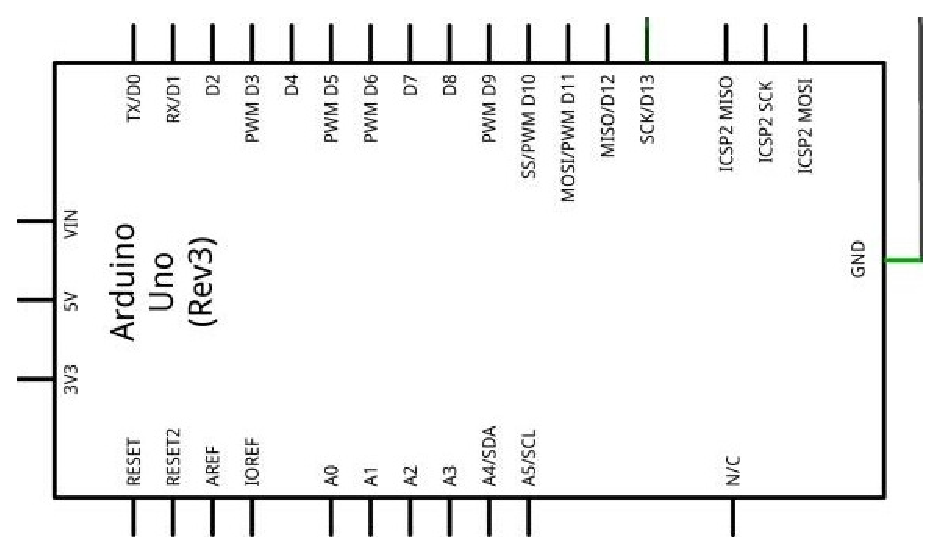
\includegraphics[scale=1]{arduino}
%\end{center}
%
\begin{problem}
	Connect the 5V pin of the arduino to an  extreme pin that is in the same segment as the 1K resistor pin. 
	\end{problem}	
\begin{problem}
	Connect the GND pin of the arduino to the opposite extreme pin of the breadboard
\end{problem}
\begin{problem}
	Connect the Arduino to the computer.
\end{problem}
\begin{problem}
	Connect the {\em dot} pin of the display to a pin in the same segment as the GND pin.  What do you observe?
\end{problem}
\subsection{Controlling the Display}
Fig. \ref{fig:sevenseg12} explains how to get decimal digits using the seven segment display. 
\begin{problem}
	Generate the number 1 on the display by connecting only the pins $b$ and $c$ to GND. 
\end{problem}	
\begin{problem}
	Repeat the above exercise to generate the number 2 on the display.
\end{problem}	
%
\begin{problem}
Table \ref{table:arduioport} summarizes the process of generating the decimal digits.  0 means connecting to ground and 1 means not connecting.  	Complete Table \ref{table:arduioport} for all numbers between 0-9.
\end{problem}	
\input{./figs/arduinoport}
%
%
\begin{figure}[!h]
\begin{center}
\resizebox {0.8\columnwidth} {!} {
\input{./figs/sevenseg12.tex}
}
\end{center}
\caption{}
\label{fig:sevenseg12}
\end{figure}
%
\begin{problem}
	Now generate all numbers between  0-9 on the display using the above table.
\end{problem}
%
%The 7447 IC helps in displaying decimal numbers on the seven segment display.  The $\bar{a}-\bar{g}$, pins of the 7447 IC are connected to the $a-g$ pins of the display. $V_{cc}$ should be connected to a 5V power source. The input pins of the decoder are A,B,C and D, with A being the lowest significant bit (LSB) and D being the most significant bit (MSB).  For example, the number 5 is visible on the display when the A,B,C and D inputs are the following.
%\begin{center}
%	\begin{tabular}{|c|c|c|c|c|}
%\hline
%D & C & B & A & Decimal
%\\ \hline
%0 & 1 & 0 & 1 & 5
%\\
%\hline
%\end{tabular}
%\end{center}
%
%%
%\begin{figure}
%\begin{center}
%\includegraphics[width=\columnwidth]{./figs/7447IC}
%\end{center}
%\caption{}
%\label{}
%\end{figure}
%
%%\begin{center}
%	%\includegraphics[scale=1.5]{7447IC}
%%\end{center}
%
%%
%\begin{problem}
%	Connect the 7447 IC decoder $\bar{a}-\bar{g}$ pins to the $a-g$ pins of the display respectively.
%\end{problem}
%\begin{problem}
%	Connect the $V_{cc}$ and GND pins of the decoder to the 5V supply and GND pins of the breadboard.
%\end{problem}
%\begin{problem}
%	Connect the A,B,C,D pins to pins in the GND extreme segment of the breadboard.  What do you observe.
%\end{problem}
%\begin{problem}
%	Now remove the D pin from the breadboard and observe the display output.
%\end{problem}
%\begin{problem}
%	Generate a table with A,B,C,D inputs and the equivalent decimal number output.
%\end{problem}

%

%\newpage
\section{Python-flask}
 Flask is Python framework for creating web applications.

\begin{enumerate}[label=\thesection.\arabic*
,ref=\thesection.\theenumi]

\item Installation:
\begin{lstlisting}
sudo apt-get update
sudo apt-get install python-pip
sudo pip install flask
\end{lstlisting}


%\begin{description}
\item {Calculator UI in HTML}:
Download the following code  and open it using a browser.  You 
will see the calculator UI.

\item Save \textbf{calc.html} in a folder called \textbf{templates}.
%\textbf{ Python Connector from Browser to Database}:

\item Type the following code in a file called \textbf{calc\_ui.py}.

\item Make sure that the python file is outside the \textbf{templates} directory.  Now type
\begin{lstlisting}
python calc_ui.py
\end{lstlisting}
on the terminal. An address will be displayed on the terminal.
\item Enter the above address in a browser.  You should see the calculator UI.
%\item As soon as you hit the submit buttom message will be displayed Data has been stored.
\end{enumerate}

\section{Python Engine}

\begin{enumerate}[label=\thesection.\arabic*
,ref=\thesection.\theenumi]
\item Write a program to concatenate 2 strings.
\\
\solution
\lstinputlisting[language=Python]{./codes/p1.py}

\item Write a program to concatenate 3 strings.
\label{item:cat}
\item Use the \textbf{eval} function in python to add, subtract, multiply and divide
two numbers using Problem \ref{item:cat}
\\
\solution
\lstinputlisting[language=Python]{./codes/add_eval.py}

\end{enumerate}

\subsection{Fetching the stored Data from the Database}
\begin{enumerate}
%\item Now we want to fetch the data that has been stored into the database.In order to this we will make one more HTML file(display.html).This file will Help to display the fetched data in a way that we want.
%\item 
%\begin{description}
\item Save the following code in a file called \textbf{display.html}.
\lstinputlisting[language=HTML]{./codes/display.html}
%\end{description}

\item %Make a python file that connect database and fetch all the Value from the particular table.
Save the following code in a file titled  \textbf{display.py}.    
%\begin{description}
\item \lstinputlisting[language=Python]{./codes/display.py}
%\end{description}

\item Now open the terminal and type 
\begin{lstlisting}
python display.py
\end{lstlisting}
An address will be displayed.
\item Open this address in a browser. You can see all the Name and Roll No entries in the database.
\end{enumerate}
\subsection{Updating the Database}
\begin{enumerate}
\item 
%Now we will create one more python file and Html file in order to update the already stored data.
    
%\begin{description}
\item Save the following code in a file with titled \textbf{show.html}.
\lstinputlisting[language=HTML]{./codes/show.html}

%\end{description}
\item Save the following code in a file titled \textbf{update.py}.
%begin{description}
\item \lstinputlisting[language=Python]{./codes/update.py}
%\end{description}
\item Now open the terminal and run the \textbf{update.py} file.
\item Update whatever data you wish to and click the Update button.
\item Run \textbf{display.py} to verify that your data is indeed updated.
%Here now you can update whatever you want to update. Just change the thing and click on update button. Data will be updated.
\end{enumerate}
\subsection{Linking all modules to create the Database application}
\begin{enumerate}
%\item Now we combine all the code in one file and will link them with each other.we will make onehtml file output.html and main python file that is app.py.
%\item For html file write below code:-
%\begin{description}
\item Save the following code in a file called \textbf{output.html}.

\lstinputlisting[language=HTML]{./codes/output.html}
%\end{description}
\item Save the following code in a file titled \textbf{app.py}
%\begin{description}
\lstinputlisting[language=Python]{./codes/app.py}
%\end{description}
\item Run \textbf{app.py}
\item Start using your application.
\item Modify your application so that you may delete a record.
\end{enumerate}


%\subsection{Powering the Display}
The breadboard can be divided into 5 segments.  In each of the green segements, the pins are internally connected so as to have the same voltage.  Similarly, in the central segments, the pins in each column  are internally connected in the same fashion as the blue columns. 

\begin{problem}
	Plug the display to the breadboard in Fig. \ref{fig:breadboard}
\end{problem}
\begin{figure}[!h]
\begin{center}
\includegraphics[width=\columnwidth]{./figs/breadboard}
\end{center}
\caption{}
\label{fig:breadboard}
\end{figure}

The seven segment display in Fig. \ref{fig:sevenseg} has eight pins, $a, b, c, d, e, f, g$ and $dot$ that take an active LOW input, i.e.  the LED will glow only if the input is connected to ground.  Each of these pins is connected to an LED segment.  The $dot$ pin is  reserved for the $\cdot$ LED.  

%
%\begin{center}
	%\includegraphics[scale=1]{sevenseg}
%\end{center}

\begin{problem}
	Connect one end of the resistor to the COM pin of the display and the other end to an extreme pin of the breadboard.	
\end{problem}
%
%
%
\begin{figure}[!h]
\begin{center}
\resizebox {0.5\columnwidth} {!} {
\input{./figs/sevenseg.tex}
}
\end{center}
\caption{}
\label{fig:sevenseg}
\end{figure}

The Arduino Uno has some ground pins, analog input pins A0-A3 and digital pins D1-D13 that can be used for both input as well as output. It also has two power pins that can generate 3.3$V$ and 5$V$.  In the following exercises, only the GND, 5$V$ and digital pins will be used.
%
%\begin{center}
	%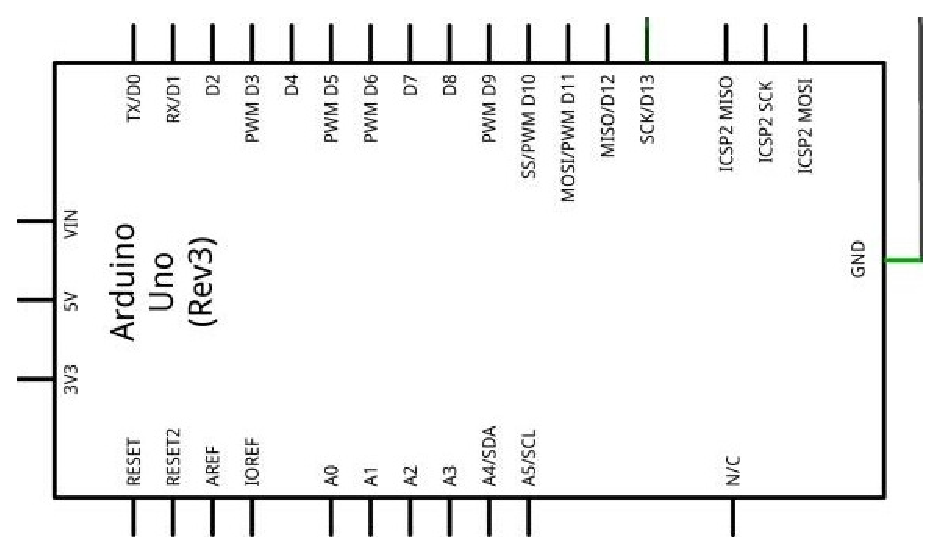
\includegraphics[scale=1]{arduino}
%\end{center}
%
\begin{problem}
	Connect the 5V pin of the arduino to an  extreme pin that is in the same segment as the 1K resistor pin. 
	\end{problem}	
\begin{problem}
	Connect the GND pin of the arduino to the opposite extreme pin of the breadboard
\end{problem}
\begin{problem}
	Connect the Arduino to the computer.
\end{problem}
\begin{problem}
	Connect the {\em dot} pin of the display to a pin in the same segment as the GND pin.  What do you observe?
\end{problem}
\subsection{Controlling the Display}
Fig. \ref{fig:sevenseg12} explains how to get decimal digits using the seven segment display. 
\begin{problem}
	Generate the number 1 on the display by connecting only the pins $b$ and $c$ to GND. 
\end{problem}	
\begin{problem}
	Repeat the above exercise to generate the number 2 on the display.
\end{problem}	
%
\begin{problem}
Table \ref{table:arduioport} summarizes the process of generating the decimal digits.  0 means connecting to ground and 1 means not connecting.  	Complete Table \ref{table:arduioport} for all numbers between 0-9.
\end{problem}	
\input{./figs/arduinoport}
%
%
\begin{figure}[!h]
\begin{center}
\resizebox {0.8\columnwidth} {!} {
\input{./figs/sevenseg12.tex}
}
\end{center}
\caption{}
\label{fig:sevenseg12}
\end{figure}
%
\begin{problem}
	Now generate all numbers between  0-9 on the display using the above table.
\end{problem}
%
%The 7447 IC helps in displaying decimal numbers on the seven segment display.  The $\bar{a}-\bar{g}$, pins of the 7447 IC are connected to the $a-g$ pins of the display. $V_{cc}$ should be connected to a 5V power source. The input pins of the decoder are A,B,C and D, with A being the lowest significant bit (LSB) and D being the most significant bit (MSB).  For example, the number 5 is visible on the display when the A,B,C and D inputs are the following.
%\begin{center}
%	\begin{tabular}{|c|c|c|c|c|}
%\hline
%D & C & B & A & Decimal
%\\ \hline
%0 & 1 & 0 & 1 & 5
%\\
%\hline
%\end{tabular}
%\end{center}
%
%%
%\begin{figure}
%\begin{center}
%\includegraphics[width=\columnwidth]{./figs/7447IC}
%\end{center}
%\caption{}
%\label{}
%\end{figure}
%
%%\begin{center}
%	%\includegraphics[scale=1.5]{7447IC}
%%\end{center}
%
%%
%\begin{problem}
%	Connect the 7447 IC decoder $\bar{a}-\bar{g}$ pins to the $a-g$ pins of the display respectively.
%\end{problem}
%\begin{problem}
%	Connect the $V_{cc}$ and GND pins of the decoder to the 5V supply and GND pins of the breadboard.
%\end{problem}
%\begin{problem}
%	Connect the A,B,C,D pins to pins in the GND extreme segment of the breadboard.  What do you observe.
%\end{problem}
%\begin{problem}
%	Now remove the D pin from the breadboard and observe the display output.
%\end{problem}
%\begin{problem}
%	Generate a table with A,B,C,D inputs and the equivalent decimal number output.
%\end{problem}

%
%\section{Display Control through Arduino Software}
%%\subsection{Driving the Segments}
\begin{problem}
Connect the $a-g$ pins of the display to the pins D2-D8 of the Arduino.
\end{problem}	
%
\begin{problem}
Open the arduino software.  Check if the ports show Arduino Uno and click the appropriate button.  
\end{problem}
\begin{problem}
\label{prob:first_code}
Type the following code and execute. What do you observe?
\lstinputlisting[language=C]{./codes/ard_dec_drive/src/main.cpp}
%// the setup function runs once when you press reset or power the board
int a=1,b=0,c=0,d=1,e=1,f=1,g=1;
void setup() {
    pinMode(2, OUTPUT);  
    pinMode(3, OUTPUT);
    pinMode(4, OUTPUT);
    pinMode(5, OUTPUT);
    pinMode(6, OUTPUT);
    pinMode(7, OUTPUT);
    pinMode(8, OUTPUT);            
}

// the loop function runs over and over again forever
void loop() {
  
  digitalWrite(2, a); 
  digitalWrite(3, b); 
  digitalWrite(4, c); 
  digitalWrite(5, d); 
  digitalWrite(6, e); 
  digitalWrite(7, f);     
  digitalWrite(8, g); 
}


\end{problem}
\begin{problem}
Now generate the numbers 0-9 by modifying the above program.
\end{problem}
%
%\newpage

%\section{Combinational Logic}
%
%\subsection{Counting Decoder}
%%
%\begin{problem}
%	\label{counter_dec}
%	In the  truth table in Table \ref{table:counter_decoder},  $W,X,Y,Z$ are the inputs
%and $A,B,C,D$ are the outputs. This table represents the system that increments the numbers 0-8 by 1 and resets the number 9 to 0
%%
%Note that  $D = 1$ for the inputs $0111$ and $1000$.  Using {\em boolean} logic,
%%
%\begin{equation}
%\label{bool_logic}
%D = WXYZ^{'} + W^{'}X^{'}Y^{'}Z
%\end{equation}
%%
%Note that $0111$ results in the expression $WXYZ^{'}$ and $1000$ yields $W^{'}X^{'}Y^{'}Z$. 
%
%Write the boolean logic functions for $A,B,C$ in terms of $W,X,Y,Z$.
%\end{problem}
%%
%\input{./figs/counter_decoder}
%The $\&\&$ operand is used for the boolean AND (multiplication) operation, the $||$ operand is used for the OR (addition) operation and the ! operand is used for the NOT ($^{'}$) operation in Arduino code.  For example, the expression for \eqref{bool_logic} in Arudino is
%\begin{verbatim}
%D = (W&&X&&Y&&!Z)||(!W&&!X&&!Y&&Z);
%\end{verbatim}
%%
%\begin{problem}
%Write the Arduino code for the outputs $A,B,C$ and verify if your logic is correct by observing the output on the seven segment display.
%\end{problem}
%%
%\subsection{Display Decoder}
%%
%\begin{problem}
%Now write the truth table for the seven segment display decoder (IC 7447).  The inputs will be $A,B,C,D$ and the outputs will be $a,b,c,d,e,f,g$.
%\end{problem}
%%
%\begin{problem}
%\label{seven_seg_disp_logic}
%Obtain the logic functions for outputs $a,b,c,d,e,f,g$ in terms of the inputs $A,B,C,D$.
%\end{problem}
%\begin{problem}
%Disconnect the arduino from IC 7447 and connect the pins D2-D8 in the Arduino directly to the seven segment display.
%\end{problem}
%\begin{problem}
%Write a new program to implement the logic in Problem \ref{seven_seg_disp_logic} and observe the output in the display.  You have designed the logic for IC 7447!
%\end{problem}
%\begin{problem}
%Now include your counting decoder program in the  display decoder program
%and see if the display shows the consecutive number.
%\end{problem}
%A decade counter counts the numbers from 0-9 and then resets to 0.
\begin{problem}
Suitably modify the above program to obtain a decade counter.
\end{problem}




%\begin{problem}
%Generate the boolean functions for the segments $a-f$ using the table in Problem \ref{bcd_ss}.  For example, the function for $a$ is obtained from the table as
%\begin{equation}
%a=\bar{D}\bar{C}\bar{B}A+\bar{D}C\bar{B}\bar{A}
%\label{boolean}
%\end{equation}
%\end{problem}
%%
%\begin{problem}
	%\label{counter_dec}
%Write functions for $A,B,C,D$ in Arduino using the following table and verify using the Arduino driven display.
		%\input{counter_decoder}
%\end{problem}
%\begin{problem}
	%Write a module for decimal to binary conversion
	%according to the example given below
	%\input{conversion}
	%%
	%$N \% 2$ gives the remainder and $N/2$ gives the quotient
%	and use it in the above code so that decimal values are given as input in the program and observed as output in the display. Note that the following code
%	\begin{verbatim}
%	a % b
%	\end{verbatim}
%	can be used to obtain the remainder when a is divided by b and
%	\begin{verbatim}
%	a/b
%	\end{verbatim}
%	gives the quotient.
%\end{problem}

%%
%\section{Decade Counter through Arduino}
%\subsection{Angle Bisectors}

\begin{figure}[!ht]
	\begin{center}
		
		%
\includegraphics[width=\columnwidth]{./figs/ch3_angle_bisector}
		%\vspace*{-10cm}
		\resizebox{\columnwidth}{!}{\input{./figs/fig_3.0.tex}}
	\end{center}
	\caption{Angle bisectors meet at a point}
	\label{ch3_angle_bisector}	
\end{figure}

\begin{definition}
	In Fig. \ref{ch3_angle_bisector}, $OB$ divides the  $\angle B$ into half, i.e.\begin{equation}
	\angle OBC = \angle OBA
	\end{equation}
	$OB$ is known as an angle bisector.
\end{definition}
	$OB$ and $OC$ are angle bisectors of angles $B$ and $C$. $OA$ is joined and $OD, OF$ and $OE$ are perpendiculars to sides $a,b$ and $c$.
\begin{problem}
  Show that $OD = OE = OF$.
\end{problem}
\proof In $\Delta$s $ODC$ and $OEC$,
\begin{align}
OD &= OC \sin \frac{C}{2}
\\
OE &= OC \sin \frac{C}{2} 
\\
\Rightarrow OD &=OE.
\end{align}
Similarly,
\begin{equation}
OD = OF.
\end{equation}
%
\begin{problem}
	Show that OA is the angle bisector of $\angle A$
\end{problem}
\proof In $\Delta$s $OFA$ and $OEA$,
\begin{align}
OF &= OE
\\
\Rightarrow OA \sin OAF &= OA \sin OAE \\
\Rightarrow \sin OAF &=  \sin OAE \\
\Rightarrow \angle OAF &= \angle OAE
\end{align}
which proves that $OA$ bisects $\angle A$.
{\em Conclusion:} The angle bisectors of a triangle meet at a point.


\subsection{Congruent Triangles}
%
\begin{problem}
	Show that in $\Delta$s $ODC$ and $OEC$, corresponding sides and angles are equal.
\end{problem}
\begin{definition}
	Note that    $\Delta$s $ODC$ and $OEC$ are known as congruent triangles.  To show that two triangles are congruent, it is sufficient to show that some angles and sides are equal.
\end{definition}
\begin{problem}
SSS:	Show that if the corresponding sides of three triangles are equal, the triangles are congruent.
\end{problem}
\begin{problem}
ASA:	Show that if two angles and any one side  are equal in corresponding triangles, the triangles are congruent.
\end{problem}
\begin{problem}
SAS:	Show that if two sides and the angle between them are equal in corresponding triangles, the triangles are congruent.
\end{problem}
\begin{problem}
RHS:	For two right angled triangles, if the hypotenuse and one of the sides are equal, show that the triangles are congruent.
\end{problem}
	%
%%
\subsection{Perpendicular Bisectors}
\begin{definition}
	In Fig. \ref{ch3_perp_bisector}, OD $\perp BC$ and $BD=DC$. $OD$ is defined as the perpendicular bisector of $BC$.
\end{definition}

\begin{problem}
	In Fig. \ref{ch3_perp_bisector}, show that $OA=OB=OC$.
\end{problem}
%%
%%
\begin{figure}[!ht]
	\begin{center}
		
		\includegraphics[width=\columnwidth]{./figs/fig_3.8.eps}
%		
\includegraphics[width=\columnwidth]{./figs/ch3_perp_bisector}
		%\vspace*{-10cm}
%		\resizebox{\columnwidth}{!}{\input{./figs/fig_3.8.tex}}
	\end{center}
	\caption{Perpendicular bisectors meet at a point}
	\label{ch3_perp_bisector}	
\end{figure}
%
\proof In $\Delta$s $ODB$ and $ODC$, using Budhayana's theorem,
%
\begin{equation}
\begin{split}
OB^2 &= OD^2 + BD^2 \\
OC^2 &= OD^2 + DC^2 
\end{split}
\end{equation}
%
Since $BD = DC = \frac{a}{2}$, $OB = OC$.  Similarly, it can be shown that $OA = OC$.  Thus, $OA=OB=OC$.
%
\begin{definition}
	In $\Delta AOB$, $OA = OB$.  Such a triangle is known as an isoceles triangle.
\end{definition}
%
\begin{problem}
	Show that $AF = BF$.
\end{problem}
\proof Trivial using Budhayana's theorem.  This shows that $OF$ is a perpendicular bisector of $AB$. 
{\em Conclusion:}  The perpendicular bisectors of a triangle meet at a point.
%
\subsection{Perpendiculars from Vertex to Opposite Side}
	%
	%
	In Fig. \ref{ch3_perp_triang}, $AD \perp BC$ and $BE \perp AC$. $CF$ passes through $O$ and meets
	$AB$ at $F$.  	
\begin{problem}
	Show that 
	\begin{align}
	OE = c \cos A \cot C
	\end{align}
\end{problem}
	\begin{figure}[!ht]
		\begin{center}
			
			%
\includegraphics[width=\columnwidth]{./figs/ch3_perp_triang}
			%\vspace*{-10cm}
			\resizebox{\columnwidth}{!}{\input{./figs/fig_3.10.tex}}
		\end{center}
		\caption{Perpendiculars from vertex to opposite side meet at a point}
		\label{ch3_perp_triang}	
	\end{figure}
%
\proof In $\Delta$ s $AEB$ and $AEO$,
%
\begin{align}
AE &= c \cos A \\
OE &= AE \tan \brak{90^{\degree} - C} \brak{\because ADC \text{ is right angled}} \\
&= AE \cot C
\end{align}
%
From both the above, we get the desired result.
%
\begin{problem}
	Show that $\alpha = A$.
\end{problem}
\proof In $\Delta OEC$,
%
\begin{equation}
CE = a \cos C \brak{\because BEC \text{ is right angled}}
\end{equation}
%
Hence,
%
\begin{equation}
\begin{split}
\tan \alpha &= \frac{CE}{OE} \\
&=  \frac{a \cos C}{c \cos A \cot C} \\
&=  \frac{a \cos C \sin C}{c \cos A \cos C} \\
&= \frac{a \sin C}{c \cos A } \\
&= \frac{c \sin A}{c \cos A } \brak{\because \frac{a}{\sin A} = \frac{c}{\sin C}}\\
&= \tan A\\
\Rightarrow \alpha = A
\end{split}
\end{equation}
%
\begin{problem}
	Show that $CF \perp AB$
\end{problem}
\proof Consider triangle OFB and the result of the previous problem.  $\because$ the sum of the angles of a triangle is $180^{\degree}$, $\angle CFB = 90^{\degree}$.
{\em Conclusion: The perperdiculars from the vertex of a triangle to the opposite side meet at a point.}
%%%
%\section{Karnaugh Maps}
%\subsection{Chord of a Circle}
%
\renewcommand{\theequation}{\theenumi}
\begin{enumerate}[label=\arabic*.,ref=\thesubsection.\theenumi]
\numberwithin{equation}{enumi}
%
\item
	Fig. \ref{ch4_circle_def} represents a circle.  The points in the circle are at a distance $r$ from the centre $O$.  $r$ is known as the radius.

\begin{figure}[!ht]
	\begin{center}
		
		%
\includegraphics[width=\columnwidth]{./figs/ch4_circle_def}
		%\vspace*{-10cm}
		\resizebox{\columnwidth}{!}{\input{./figs/fig_4.0.tex}}
	\end{center}
	\caption{Circle Definitions}
	\label{ch4_circle_def}	
\end{figure}
\end{enumerate}
\subsection{Chords of a circle}
%
\renewcommand{\theequation}{\theenumi}
\begin{enumerate}[label=\arabic*.,ref=\thesubsection.\theenumi]
\numberwithin{equation}{enumi}
%
\item
	In Fig. \ref{ch4_circle_def}, $A$ and $B$ are points on the circle.  The line $AB$ is known as a chord of the circle.

%
%
\item
	\label{ch4_prob_circle_subtend}
	In Fig. \ref{ch4_circle_subtend}  Show that $\angle AOB = 2\angle ACB $.

\begin{figure}[!ht]
	\begin{center}
		
		%
\includegraphics[width=\columnwidth]{./figs/ch4_circle_subtend}
		%\vspace*{-10cm}
		\resizebox{\columnwidth}{!}{\input{./figs/fig_4.1.tex}}
	\end{center}
	\caption{Angle subtended by chord $AB$ at the centre $O$ is twice the angle subtended at $P$. }
	\label{ch4_circle_subtend}	
\end{figure}

\solution In Fig. \ref{ch4_circle_subtend}, the triangeles $OPA$ and $OPB$ are isosceles. Hence,
%
\begin{align}
\angle OCA = \angle OAC &= \theta_1 \\
\angle OCB = \angle OBC &= \theta_2
\end{align}
%
Also, $\alpha$ and $\beta$ are exterior angles corresponding to the triangle $AOC$ and $BOC$ respectively. Hence
%
\begin{align}
\alpha &= 2\theta_1 \\
\beta &= 2\theta_2
\end{align}
%
Thus,
%
\begin{align}
\angle AOB &= \alpha + \beta \\
&= 2\brak{\theta_1 + \theta_2} \\
&= 2\angle ACB
\end{align}
%
\item
	The diameter of a circle is the chord that divides the circle into two equal parts. In Fig. \ref{ch4_circle_dia}, $AB$ is the diameter and passes through the centre $O$

%
\item
In Fig. \ref{ch4_circle_dia}, show that $\angle APB = 90^{\degree}$ .

%
\begin{figure}[!ht]
	\begin{center}
		
		%
\includegraphics[width=\columnwidth]{./figs/ch4_circle_dia}
		%\vspace*{-10cm}
		\resizebox{\columnwidth}{!}{\input{./figs/fig_4.2.tex}}
	\end{center}
	\caption{Diameter of a circle.}
	\label{ch4_circle_dia}	
\end{figure}
\item
	In Fig. \ref{ch4_chord_product}, show that 
	\begin{equation}
	\begin{split}
\angle ABD &= \angle ACD \\
\angle CAB &= \angle CDB	
	\end{split}
	\end{equation}

\begin{figure}[!ht]
	\begin{center}
		
		%
\includegraphics[width=\columnwidth]{./figs/ch4_chord_product}
		%\vspace*{-10cm}
		\resizebox{\columnwidth}{!}{\input{./figs/fig_4.3.tex}}
	\end{center}
	\caption{$PA.PB = PC.PD$}
	\label{ch4_chord_product}	
\end{figure}
%
%
\solution Use Problem \ref{ch4_prob_circle_subtend}.
%
\item
	In Fig. \ref{ch4_chord_product}, show that the triangles $PAB$ and $PBD$ are similar

\solution Trivial using previous problem
\item
	In Fig. \ref{ch4_chord_product}, show that 
	\begin{equation}
	PA.PB = PC.PD
	\end{equation}

%
\solution Since triangles $PAC$ and $PBD$ are similar, 
%
\begin{align}
\frac{PA}{PD} &= \frac{PC}{PB} \\
\Rightarrow PA.PB &= PC.PD
\end{align}
%
%
\item
	Show that 
	\begin{equation}
	\label{ch5_sin_zero}
	\sin 0^{\degree} = 0
	\end{equation}

\solution Follows from \eqref{ch5_sin_increasing}.
%
\item
	Show that 
	\begin{equation}
	\label{ch5_sin_zero}
	\cos 0^{\degree} = 1
	\end{equation}
	
\item
	The line $PX$ in Fig. \ref{ch4_tangent_def} touches the circle at exactly one  point $P$. It is known as the tangent to the circle.

%
%
\item
	Show that $OP \perp PX$.
% is the perpendicular to the line $PX$ as shown in the Fig. \ref{ch4_short_dist}. Show that $OP$ is the shortest distance between the point $O$ and the line $PX$. 

\solution Without loss of generality, let $0 \le \theta \le 90^{\degree}$. Using the cosine formula in $\triangle OPP_n$,\begin{align}
\brak{r+d_n}^2 > r^2,
\end{align}
%Let $P_1$ be a point on the line $PX$. Then $OPP_1$ is a right angled triangle.  Using Budhayana's theorem,
%
\begin{figure}[!ht]
	\begin{center}
		
		%
\includegraphics[width=\columnwidth]{./figs/ch4_tangent_def}
		%\vspace*{-10cm}
		\resizebox{\columnwidth}{!}{\begin{tikzpicture}
[scale =2,>=stealth,point/.style = {draw, circle, fill = black, inner sep = 1pt},]

\def\rad{2}
\coordinate [point, label={right: $O$ }] (O) at (0, 2);
\draw (O) circle (\rad);
\node (P) at (0,0)[point,label=below :$P$] {};
\node (X) at (2,0)[point,label=right :$X$] {};
\node (Y) at (-4,0)[point,label=left :$Y$] {};
\node (P_1) at (-1,0)[point,label=below  :$P_1$] {};
\node (P_2) at (-2,0)[point,label=below  :$P_2$] {};
\node (P_3) at (-3,0)[point,label=below  :$P_3$] {};

\draw (O)--(P);
\draw (X)--(Y);
\draw (O)--(P_1);
\draw (O)--(P_2);
\draw (O)--(P_3);

\tkzMarkRightAngle[size=.2](O,P,P_1);
\node [above] at (-0.8,0.5){$r$};
\node [above] at (-1.2,0.8){$r$};
\node [above] at (-1.45,1){$r$};
\node [above] at (0.1,0.8){$r$};
\end{tikzpicture}}
	\end{center}
	\caption{Tangent to a Circle.}
	\label{ch4_tangent_def}	
\end{figure}
%
%\begin{figure}[!ht]
%	\begin{center}
%		
%		%
\includegraphics[width=\columnwidth]{./figs/ch4_short_dist}
%		%\vspace*{-10cm}
%		\resizebox{\columnwidth}{!}{\input{./figs/fig_4.6_1.tex}}
%	\end{center}
%	\caption{Shortest distance from $O$ to line $PX$}
%	\label{ch4_short_dist}	
%\end{figure}

%
\begin{align}
%\begin{split}
\brak{r+d_n}^2 = r^2 + x_n^2 - 2rx_n\cos\theta > r^2 
\\
\implies  0 <\cos\theta < \frac{x_n}{2r},
%OP_1^2 &= OP^2 + PP_1^2 \\
%\Rightarrow OP_1 > OP
%\end{split}
\end{align}
%
where $x_n$ can be made as small as we choose.  Thus, 
%
\begin{align}
\cos \theta = 0 \implies \theta  = 90 ^{\degree}.
\end{align}

%\solution In Fig. \ref{ch4_tangent_def}, we can see that $OP$ is is the radius of the circle and the length of all line segments from $O$ to the line $PX > r$.  Using the result of the previous 
%problem, it is obvious that $OP \perp PX$. 
%
	%
\item
In Fig. \ref{ch4_tangent_prod} show that 
%
\begin{equation}
\angle PCA = \angle PBC
\end{equation}
%
$O$ is the centre of the circle and $PC$ is the tangent.

	\begin{figure}[!ht]
		\begin{center}
			
			%
\includegraphics[width=\columnwidth]{./figs/ch4_tangent_prod}
			%\vspace*{-10cm}
			\resizebox{\columnwidth}{!}{\input{./figs/fig_4.8.tex}}
		\end{center}
		\caption{$PA.PB = PC^2$.}
		\label{ch4_tangent_prod}	
	\end{figure}
	%

%
\solution Obvious from the figure once we observe that $\triangle OAC$ is isosceles.
%
%
\item
	In Fig. \ref{ch4_tangent_prod}, show that the triangles $PAC$ and $PBC$ are similar.

\solution From the previous problem, it is obvious that corresponding angles of both triangles are equal.  Hence they are similar.
%
\item
	Show that $PA.PB = PC^2$

\solution Since $\Delta PAC \sim \Delta PBC$, their sides are in the same ratio.  Hence,
%
\begin{align}
\frac{PA}{PC} &= \frac{PC}{PB} \\
\Rightarrow PA.PB &=PC^2
\end{align}
%
\item
Given that $PA.PB = PC^2$, show that $PC$ is a tangent to the circle.

%
\item
	In Fig. \ref{ch4_chord_tangent_prod}, show that\begin{equation}
	PA.PB = PC.PD
	\end{equation}

%
\begin{figure}[!ht]
	\begin{center}
		
		%
\includegraphics[width=\columnwidth]{./figs/ch4_chord_tangent_prod}
		%\vspace*{-10cm}
		\resizebox{\columnwidth}{!}{\input{./figs/fig_4.11.tex}}
	\end{center}
	\caption{$PA.PB = PC^2$.}
	\label{ch4_chord_tangent_prod}	
\end{figure}

\solution Draw a tangent and use the previous problem.
\end{enumerate}

%%
%\section{Sequential Logic}
%\subsection{Area of a Circle}
%
%
\renewcommand{\theequation}{\theenumi}
\begin{enumerate}[label=\arabic*.,ref=\thesubsection.\theenumi]
\numberwithin{equation}{enumi}
%

\item
	In Fig. \ref{ch5_polygon_def}, 6 congruent triangles are arranged in a circular fashion.  Such a figure is known as a regular hexagon.  In general, $n$ number of traingles can be arranged to form a regular polygon.
\begin{figure}[!ht]
	\begin{center}
		
		%
\includegraphics[width=\columnwidth]{./figs/ch5_polygon_def}
		%\vspace*{-10cm}
		\resizebox{\columnwidth}{!}{\input{./figs/fig_5.0.tex}}
	\end{center}
	\caption{Polygon Definition}
	\label{ch5_polygon_def}	
\end{figure}
%
\item
The angle formed by each of the congruent triangles at the centre of a regular polygon of $n$ sides is $\frac{360^{\degree}}{n}$.

%
\item
Show that the area of a regular polygon is given by 
%
\begin{equation}
\frac{n}{2}r^{2}\sin\frac{360^{\degree}}{n}
\end{equation}
%

\begin{figure}[!ht]
	\begin{center}
		
		%
\includegraphics[width=\columnwidth]{./figs/ch5_polygon_area}
		%\vspace*{-10cm}
		\resizebox{\columnwidth}{!}{\input{./figs/fig_5.1.tex}}
	\end{center}
	\caption{Polygon Area}
	\label{ch5_polygon_area}	
\end{figure}
%

\solution The triangle that forms the polygon of $n$ sides is given in Fig. \ref{ch5_polygon_area}.  Thus,
%
\begin{equation}
\begin{split}
ar\brak{polygon} &= n \times ar\brak{\Delta ABC} \\
&= \frac{n}{2}r^{2}\sin\frac{360^{\degree}}{n}
\end{split}
\end{equation}
%
\item
	Using Fig. \ref{ch5_circle_squeeze}, show that
%
\begin{equation}
\label{ch5_circle_squeeze_eq}
\frac{n}{2}r^{2}\sin\frac{360^{\degree}}{n} < \text{ area of circle } < nr^{2}\tan\frac{180^{\degree}}{n}
\end{equation}
%
The portion of the circle visible in Fig. \ref{ch5_circle_squeeze} is defined to be a sector of the circle.

\begin{figure}[!ht]
	\begin{center}
		
		%
\includegraphics[width=\columnwidth]{./figs/ch5_circle_squeeze}
		%\vspace*{-10cm}
		\resizebox{\columnwidth}{!}{\input{./figs/fig_5.2.tex}}
	\end{center}
	\caption{Circle Area in between Area of Two Polygons}
	\label{ch5_circle_squeeze}	
\end{figure}
%

\solution Note that the circle is squeezed between the inner and outer regular polygons.  As we can see from Fig. \ref{ch5_circle_squeeze}, the area of the circle should be in between the areas of the inner and outer polygons.  Since
%
\begin{align}
ar \brak{\Delta OAB} &= \frac{1}{2}r^{2}\sin\frac{360^{\degree}}{n} \\
ar \brak{\Delta OPQ} &= 2 \times \frac{1}{2} \times r \tan\frac{360/n}{2} \times r \\
&= r^{2}\tan\frac{180^{\degree}}{n},
\end{align}
%
we obtain \eqref{ch5_circle_squeeze_eq}.
%
%
\item
	Using Fig. \ref{ch5_sin_theta}, show that 
	%
\begin{equation}
\label{ch5_sin_theta_eq}
\sin  \theta_1 = \sin \brak{\theta_1 + \theta_2}\cos \theta_2 - \cos\brak{\theta_1+\theta_2}\sin\theta_2
\end{equation}	
	%

\begin{figure}[!ht]
	\begin{center}
		
		%
\includegraphics[width=\columnwidth]{./figs/ch5_sin_theta}
		%\vspace*{-10cm}
		\resizebox{\columnwidth}{!}{\input{./figs/fig_5.3.tex}}
	\end{center}
	\caption{$\sin2\theta = 2\sin\theta\cos\theta$}
	\label{ch5_sin_theta}	
\end{figure}
%

\solution The following equations can be obtained from the figure using the forumula for the area of a triangle
%
\begin{align}
ar \brak{\Delta ABC} &= \frac{1}{2}ac \sin\brak{\theta_1 + \theta_2} \\
&= ar \brak{\Delta BDC} + ar \brak{\Delta ADB} \\
&= \frac{1}{2}cl \sin{\theta_1} + \frac{1}{2}al \sin{\theta_2} \\ 
&= \frac{1}{2}ac \sin{\theta_1} \sec \theta_2 + \frac{1}{2}a^2 \tan{\theta_2} 
\end{align}
$\brak{\because
	l = a \sec \theta_2}$.  From the above,
\begin{align}
\Rightarrow \sin\brak{\theta_1 + \theta_2} &=  \sin{\theta_1} \sec \theta_2 + \frac{a}{c} \tan{\theta_2} \\
\Rightarrow \sin\brak{\theta_1 + \theta_2} &=  \sin{\theta_1} \sec \theta_2 + \cos\brak{\theta_1 + \theta_2} \tan{\theta_2} 
\end{align}
Multiplying both sides by $\cos \theta_2$,
\begin{align}
\Rightarrow \sin\brak{\theta_1 + \theta_2}\cos{\theta_2} &=  \sin{\theta_1}  + \cos\brak{\theta_1 + \theta_2} \sin\theta_2  
\end{align}
%
resulting in
\begin{equation}
\Rightarrow \sin \theta_1 = \sin\brak{\theta_1 + \theta_2}\cos{\theta_2} - \cos\brak{\theta_1 + \theta_2} \sin\theta_2 
\end{equation}
\item
	Prove the following identities 
	%
	\begin{enumerate}
\item 
\begin{equation}
		\label{ch5_sin_diff}
\sin\brak{\alpha - \beta} = \sin \alpha \cos \beta - \cos \alpha \sin \beta.
\end{equation}
\item 
\begin{equation}
\cos\brak{\alpha + \beta} = \cos \alpha \cos \beta - \sin \alpha \sin \beta.
		\label{ch5_cos_diff}
\end{equation}

	\end{enumerate}
	%

\solution In \eqref{ch5_sin_theta_eq}, let
%
\begin{equation}
\begin{split}
\theta_1 + \theta_2 &= \alpha \\
\theta_2 &=  \beta
\end{split}
\end{equation}
%
This gives \eqref{ch5_sin_diff}.  In \eqref{ch5_sin_diff}, replace $\alpha$ by 
%
$90^{\degree} - \alpha$.  This results in
%
\begin{multline}
\sin\brak{90^{\degree} - \alpha - \beta}
\\
=
\sin \brak{90^{\degree} -\alpha} \cos \beta - \cos \brak{90^{\degree} -\alpha} \sin \beta \\
\Rightarrow \cos\brak{\alpha + \beta} = \cos \alpha \cos \beta - \sin \alpha \sin \beta
\end{multline}
% 
\item
	Using \eqref{ch5_sin_theta_eq} and \eqref{ch5_cos_diff}, show that
\begin{align}
\label{ch5_sin_sum}
\sin\brak{\theta_1 + \theta_2} &= \sin\theta_1  \cos\theta_2 + \cos\theta_1\sin\theta_2
\\
\cos\brak{\theta_1 - \theta_2} &= \cos\theta_1  \cos\theta_2  \sin\theta_1\sin\theta_2
\label{ch5_cos_sum}
\end{align}

%
\solution From \eqref{ch5_sin_theta_eq},
%
\begin{align}
 \sin \brak{\theta_1 + \theta_2}\cos \theta_2 =\sin  \theta_1 +\cos\brak{\theta_1+\theta_2}\sin\theta_2 
\end{align}
%
Using \eqref{ch5_cos_diff} in the above,
%
\begin{multline}
\sin \brak{\theta_1 + \theta_2}\cos \theta_2 
=\sin  \theta_1 +\lbrak{\cos \theta_1\cos\theta_2 }
\\	
\rbrak{	- \sin \theta_1\sin\theta_2}\sin\theta_2 
\end{multline}
%
which can be expressed as
%
\begin{multline}
\sin \brak{\theta_1 + \theta_2}\cos \theta_2 
=\sin  \theta_1 +\cos \theta_1\cos\theta_2 \sin\theta_2 
\\	
	- \sin \theta_1\sin^2\theta_2
\end{multline}
%
Since
%
\begin{equation}
\sin^2\theta_2 = 1- \cos^2\theta_2, 
\end{equation}
%
we obtain
%
\begin{multline}
\sin \brak{\theta_1 + \theta_2}\cos \theta_2 
=\cos \theta_1\cos\theta_2 \sin\theta_2 
\\	
+ \sin \theta_1\cos^2\theta_2
\end{multline}
%
resulting in
%
\begin{equation}
\sin \brak{\theta_1 + \theta_2}
=\cos \theta_1 \sin\theta_2 
+ \sin \theta_1\cos\theta_2
\end{equation}
%
after factoring out $\cos \theta_2$.  Using a similar approach, \eqref{ch5_cos_sum} can also be proved.
%
\item
	Show that
	%
	\begin{equation}
	\label{eq:sin2theta}
	\sin 2\theta = 2 \sin\theta \cos\theta
	\end{equation}
	%

\item
Show that
	%
	\begin{equation}
	\label{ch5_circle_squeeze_simple}
\cos^2\frac{180^{\degree}}{n} < \frac{\text{ area of circle }}{nr^{2}\tan\frac{180^{\degree}}{n}} < 1	\end{equation}
	%

\solution From \eqref{ch5_circle_squeeze_eq} and \eqref{eq:sin2theta},
	%
	\begin{multline}
	\frac{n}{2}r^{2}\sin\frac{360^{\degree}}{n} < \text{ area of circle } 
	\\
	< nr^{2}\tan\frac{180^{\degree}}{n} 
	\\
\Rightarrow 	
	{n}r^{2}\sin\frac{180^{\degree}}{n}\cos\frac{180^{\degree}}{n} < \text{ area of circle } 
	\\
	< nr^{2}\tan\frac{180^{\degree}}{n} 
	\end{multline}
%
%
\item
	Show that for large values of $n$
	%
	\begin{equation}
	%
\cos^2\frac{180^{\degree}}{n} = 1
%
	\end{equation}	
	% 

%
\solution  Follows from previous problem.
%
\item
	The previous result can be expressed as
%
\begin{equation}
\lim_{n \rightarrow \infty}\cos^2\frac{180^{\degree}}{n} = 1
\end{equation}
%	

\item
	Show that 
	%
\begin{equation}
\text{ area of circle } = r^2\lim_{n \rightarrow \infty}
{n\tan\frac{180^{\degree}}{n}} 
	%
\end{equation}	
	% 

%
\item
	\begin{equation}
	\pi = \lim_{n \rightarrow \infty}
	{n\tan\frac{180^{\degree}}{n}}
	\end{equation}

Thus, the area of a circle is $\pi r^2$.
\item
	The radian is a unit of angle defined by
\begin{equation}
	1 \text{ radian} = \frac{360^{\degree}}{2\pi}
\end{equation}

%
\item
	Show that the circumference of a circle is $2 \pi r$.

\item
	Show that the area of a sector with angle $\theta$ in radians is $\frac{1}{2}r^2\theta$.

\item
	Show that
	\begin{equation}
	\lim_{\theta \rightarrow 0} \frac{\sin\theta}{\theta} = 1
	\end{equation}

\end{enumerate}

%
%\section{C Programming}
%\input{./chapters/chapter6}

%\input{arduinoport}

%\bibliography{IEEEabrv,gvv_matrix}

%%\subsection{Driving the Segments}
\begin{problem}
Connect the $a-g$ pins of the display to the pins D2-D8 of the Arduino.
\end{problem}	
%
\begin{problem}
Open the arduino software.  Check if the ports show Arduino Uno and click the appropriate button.  
\end{problem}
\begin{problem}
\label{prob:first_code}
Type the following code and execute. What do you observe?
\lstinputlisting[language=C]{./codes/ard_dec_drive/src/main.cpp}
%// the setup function runs once when you press reset or power the board
int a=1,b=0,c=0,d=1,e=1,f=1,g=1;
void setup() {
    pinMode(2, OUTPUT);  
    pinMode(3, OUTPUT);
    pinMode(4, OUTPUT);
    pinMode(5, OUTPUT);
    pinMode(6, OUTPUT);
    pinMode(7, OUTPUT);
    pinMode(8, OUTPUT);            
}

// the loop function runs over and over again forever
void loop() {
  
  digitalWrite(2, a); 
  digitalWrite(3, b); 
  digitalWrite(4, c); 
  digitalWrite(5, d); 
  digitalWrite(6, e); 
  digitalWrite(7, f);     
  digitalWrite(8, g); 
}


\end{problem}
\begin{problem}
Now generate the numbers 0-9 by modifying the above program.
\end{problem}
%
%\newpage

%\section{Combinational Logic}
%
%\subsection{Counting Decoder}
%%
%\begin{problem}
%	\label{counter_dec}
%	In the  truth table in Table \ref{table:counter_decoder},  $W,X,Y,Z$ are the inputs
%and $A,B,C,D$ are the outputs. This table represents the system that increments the numbers 0-8 by 1 and resets the number 9 to 0
%%
%Note that  $D = 1$ for the inputs $0111$ and $1000$.  Using {\em boolean} logic,
%%
%\begin{equation}
%\label{bool_logic}
%D = WXYZ^{'} + W^{'}X^{'}Y^{'}Z
%\end{equation}
%%
%Note that $0111$ results in the expression $WXYZ^{'}$ and $1000$ yields $W^{'}X^{'}Y^{'}Z$. 
%
%Write the boolean logic functions for $A,B,C$ in terms of $W,X,Y,Z$.
%\end{problem}
%%
%\input{./figs/counter_decoder}
%The $\&\&$ operand is used for the boolean AND (multiplication) operation, the $||$ operand is used for the OR (addition) operation and the ! operand is used for the NOT ($^{'}$) operation in Arduino code.  For example, the expression for \eqref{bool_logic} in Arudino is
%\begin{verbatim}
%D = (W&&X&&Y&&!Z)||(!W&&!X&&!Y&&Z);
%\end{verbatim}
%%
%\begin{problem}
%Write the Arduino code for the outputs $A,B,C$ and verify if your logic is correct by observing the output on the seven segment display.
%\end{problem}
%%
%\subsection{Display Decoder}
%%
%\begin{problem}
%Now write the truth table for the seven segment display decoder (IC 7447).  The inputs will be $A,B,C,D$ and the outputs will be $a,b,c,d,e,f,g$.
%\end{problem}
%%
%\begin{problem}
%\label{seven_seg_disp_logic}
%Obtain the logic functions for outputs $a,b,c,d,e,f,g$ in terms of the inputs $A,B,C,D$.
%\end{problem}
%\begin{problem}
%Disconnect the arduino from IC 7447 and connect the pins D2-D8 in the Arduino directly to the seven segment display.
%\end{problem}
%\begin{problem}
%Write a new program to implement the logic in Problem \ref{seven_seg_disp_logic} and observe the output in the display.  You have designed the logic for IC 7447!
%\end{problem}
%\begin{problem}
%Now include your counting decoder program in the  display decoder program
%and see if the display shows the consecutive number.
%\end{problem}
%A decade counter counts the numbers from 0-9 and then resets to 0.
\begin{problem}
Suitably modify the above program to obtain a decade counter.
\end{problem}




%\begin{problem}
%Generate the boolean functions for the segments $a-f$ using the table in Problem \ref{bcd_ss}.  For example, the function for $a$ is obtained from the table as
%\begin{equation}
%a=\bar{D}\bar{C}\bar{B}A+\bar{D}C\bar{B}\bar{A}
%\label{boolean}
%\end{equation}
%\end{problem}
%%
%\begin{problem}
	%\label{counter_dec}
%Write functions for $A,B,C,D$ in Arduino using the following table and verify using the Arduino driven display.
		%\input{counter_decoder}
%\end{problem}
%\begin{problem}
	%Write a module for decimal to binary conversion
	%according to the example given below
	%\input{conversion}
	%%
	%$N \% 2$ gives the remainder and $N/2$ gives the quotient
%	and use it in the above code so that decimal values are given as input in the program and observed as output in the display. Note that the following code
%	\begin{verbatim}
%	a % b
%	\end{verbatim}
%	can be used to obtain the remainder when a is divided by b and
%	\begin{verbatim}
%	a/b
%	\end{verbatim}
%	gives the quotient.
%\end{problem}
 
%%
%\newpage
%\section{$M$-ary Modulation}
%\subsection{Angle Bisectors}

\begin{figure}[!ht]
	\begin{center}
		
		%
\includegraphics[width=\columnwidth]{./figs/ch3_angle_bisector}
		%\vspace*{-10cm}
		\resizebox{\columnwidth}{!}{\input{./figs/fig_3.0.tex}}
	\end{center}
	\caption{Angle bisectors meet at a point}
	\label{ch3_angle_bisector}	
\end{figure}

\begin{definition}
	In Fig. \ref{ch3_angle_bisector}, $OB$ divides the  $\angle B$ into half, i.e.\begin{equation}
	\angle OBC = \angle OBA
	\end{equation}
	$OB$ is known as an angle bisector.
\end{definition}
	$OB$ and $OC$ are angle bisectors of angles $B$ and $C$. $OA$ is joined and $OD, OF$ and $OE$ are perpendiculars to sides $a,b$ and $c$.
\begin{problem}
  Show that $OD = OE = OF$.
\end{problem}
\proof In $\Delta$s $ODC$ and $OEC$,
\begin{align}
OD &= OC \sin \frac{C}{2}
\\
OE &= OC \sin \frac{C}{2} 
\\
\Rightarrow OD &=OE.
\end{align}
Similarly,
\begin{equation}
OD = OF.
\end{equation}
%
\begin{problem}
	Show that OA is the angle bisector of $\angle A$
\end{problem}
\proof In $\Delta$s $OFA$ and $OEA$,
\begin{align}
OF &= OE
\\
\Rightarrow OA \sin OAF &= OA \sin OAE \\
\Rightarrow \sin OAF &=  \sin OAE \\
\Rightarrow \angle OAF &= \angle OAE
\end{align}
which proves that $OA$ bisects $\angle A$.
{\em Conclusion:} The angle bisectors of a triangle meet at a point.


\subsection{Congruent Triangles}
%
\begin{problem}
	Show that in $\Delta$s $ODC$ and $OEC$, corresponding sides and angles are equal.
\end{problem}
\begin{definition}
	Note that    $\Delta$s $ODC$ and $OEC$ are known as congruent triangles.  To show that two triangles are congruent, it is sufficient to show that some angles and sides are equal.
\end{definition}
\begin{problem}
SSS:	Show that if the corresponding sides of three triangles are equal, the triangles are congruent.
\end{problem}
\begin{problem}
ASA:	Show that if two angles and any one side  are equal in corresponding triangles, the triangles are congruent.
\end{problem}
\begin{problem}
SAS:	Show that if two sides and the angle between them are equal in corresponding triangles, the triangles are congruent.
\end{problem}
\begin{problem}
RHS:	For two right angled triangles, if the hypotenuse and one of the sides are equal, show that the triangles are congruent.
\end{problem}
	%
%%
\subsection{Perpendicular Bisectors}
\begin{definition}
	In Fig. \ref{ch3_perp_bisector}, OD $\perp BC$ and $BD=DC$. $OD$ is defined as the perpendicular bisector of $BC$.
\end{definition}

\begin{problem}
	In Fig. \ref{ch3_perp_bisector}, show that $OA=OB=OC$.
\end{problem}
%%
%%
\begin{figure}[!ht]
	\begin{center}
		
		\includegraphics[width=\columnwidth]{./figs/fig_3.8.eps}
%		
\includegraphics[width=\columnwidth]{./figs/ch3_perp_bisector}
		%\vspace*{-10cm}
%		\resizebox{\columnwidth}{!}{\input{./figs/fig_3.8.tex}}
	\end{center}
	\caption{Perpendicular bisectors meet at a point}
	\label{ch3_perp_bisector}	
\end{figure}
%
\proof In $\Delta$s $ODB$ and $ODC$, using Budhayana's theorem,
%
\begin{equation}
\begin{split}
OB^2 &= OD^2 + BD^2 \\
OC^2 &= OD^2 + DC^2 
\end{split}
\end{equation}
%
Since $BD = DC = \frac{a}{2}$, $OB = OC$.  Similarly, it can be shown that $OA = OC$.  Thus, $OA=OB=OC$.
%
\begin{definition}
	In $\Delta AOB$, $OA = OB$.  Such a triangle is known as an isoceles triangle.
\end{definition}
%
\begin{problem}
	Show that $AF = BF$.
\end{problem}
\proof Trivial using Budhayana's theorem.  This shows that $OF$ is a perpendicular bisector of $AB$. 
{\em Conclusion:}  The perpendicular bisectors of a triangle meet at a point.
%
\subsection{Perpendiculars from Vertex to Opposite Side}
	%
	%
	In Fig. \ref{ch3_perp_triang}, $AD \perp BC$ and $BE \perp AC$. $CF$ passes through $O$ and meets
	$AB$ at $F$.  	
\begin{problem}
	Show that 
	\begin{align}
	OE = c \cos A \cot C
	\end{align}
\end{problem}
	\begin{figure}[!ht]
		\begin{center}
			
			%
\includegraphics[width=\columnwidth]{./figs/ch3_perp_triang}
			%\vspace*{-10cm}
			\resizebox{\columnwidth}{!}{\input{./figs/fig_3.10.tex}}
		\end{center}
		\caption{Perpendiculars from vertex to opposite side meet at a point}
		\label{ch3_perp_triang}	
	\end{figure}
%
\proof In $\Delta$ s $AEB$ and $AEO$,
%
\begin{align}
AE &= c \cos A \\
OE &= AE \tan \brak{90^{\degree} - C} \brak{\because ADC \text{ is right angled}} \\
&= AE \cot C
\end{align}
%
From both the above, we get the desired result.
%
\begin{problem}
	Show that $\alpha = A$.
\end{problem}
\proof In $\Delta OEC$,
%
\begin{equation}
CE = a \cos C \brak{\because BEC \text{ is right angled}}
\end{equation}
%
Hence,
%
\begin{equation}
\begin{split}
\tan \alpha &= \frac{CE}{OE} \\
&=  \frac{a \cos C}{c \cos A \cot C} \\
&=  \frac{a \cos C \sin C}{c \cos A \cos C} \\
&= \frac{a \sin C}{c \cos A } \\
&= \frac{c \sin A}{c \cos A } \brak{\because \frac{a}{\sin A} = \frac{c}{\sin C}}\\
&= \tan A\\
\Rightarrow \alpha = A
\end{split}
\end{equation}
%
\begin{problem}
	Show that $CF \perp AB$
\end{problem}
\proof Consider triangle OFB and the result of the previous problem.  $\because$ the sum of the angles of a triangle is $180^{\degree}$, $\angle CFB = 90^{\degree}$.
{\em Conclusion: The perperdiculars from the vertex of a triangle to the opposite side meet at a point.} 
%
%\newpage
%\section{BER in Rayleigh Flat Slowly Fading Channels}
%\subsection{Chord of a Circle}
%
\renewcommand{\theequation}{\theenumi}
\begin{enumerate}[label=\arabic*.,ref=\thesubsection.\theenumi]
\numberwithin{equation}{enumi}
%
\item
	Fig. \ref{ch4_circle_def} represents a circle.  The points in the circle are at a distance $r$ from the centre $O$.  $r$ is known as the radius.

\begin{figure}[!ht]
	\begin{center}
		
		%
\includegraphics[width=\columnwidth]{./figs/ch4_circle_def}
		%\vspace*{-10cm}
		\resizebox{\columnwidth}{!}{\input{./figs/fig_4.0.tex}}
	\end{center}
	\caption{Circle Definitions}
	\label{ch4_circle_def}	
\end{figure}
\end{enumerate}
\subsection{Chords of a circle}
%
\renewcommand{\theequation}{\theenumi}
\begin{enumerate}[label=\arabic*.,ref=\thesubsection.\theenumi]
\numberwithin{equation}{enumi}
%
\item
	In Fig. \ref{ch4_circle_def}, $A$ and $B$ are points on the circle.  The line $AB$ is known as a chord of the circle.

%
%
\item
	\label{ch4_prob_circle_subtend}
	In Fig. \ref{ch4_circle_subtend}  Show that $\angle AOB = 2\angle ACB $.

\begin{figure}[!ht]
	\begin{center}
		
		%
\includegraphics[width=\columnwidth]{./figs/ch4_circle_subtend}
		%\vspace*{-10cm}
		\resizebox{\columnwidth}{!}{\input{./figs/fig_4.1.tex}}
	\end{center}
	\caption{Angle subtended by chord $AB$ at the centre $O$ is twice the angle subtended at $P$. }
	\label{ch4_circle_subtend}	
\end{figure}

\solution In Fig. \ref{ch4_circle_subtend}, the triangeles $OPA$ and $OPB$ are isosceles. Hence,
%
\begin{align}
\angle OCA = \angle OAC &= \theta_1 \\
\angle OCB = \angle OBC &= \theta_2
\end{align}
%
Also, $\alpha$ and $\beta$ are exterior angles corresponding to the triangle $AOC$ and $BOC$ respectively. Hence
%
\begin{align}
\alpha &= 2\theta_1 \\
\beta &= 2\theta_2
\end{align}
%
Thus,
%
\begin{align}
\angle AOB &= \alpha + \beta \\
&= 2\brak{\theta_1 + \theta_2} \\
&= 2\angle ACB
\end{align}
%
\item
	The diameter of a circle is the chord that divides the circle into two equal parts. In Fig. \ref{ch4_circle_dia}, $AB$ is the diameter and passes through the centre $O$

%
\item
In Fig. \ref{ch4_circle_dia}, show that $\angle APB = 90^{\degree}$ .

%
\begin{figure}[!ht]
	\begin{center}
		
		%
\includegraphics[width=\columnwidth]{./figs/ch4_circle_dia}
		%\vspace*{-10cm}
		\resizebox{\columnwidth}{!}{\input{./figs/fig_4.2.tex}}
	\end{center}
	\caption{Diameter of a circle.}
	\label{ch4_circle_dia}	
\end{figure}
\item
	In Fig. \ref{ch4_chord_product}, show that 
	\begin{equation}
	\begin{split}
\angle ABD &= \angle ACD \\
\angle CAB &= \angle CDB	
	\end{split}
	\end{equation}

\begin{figure}[!ht]
	\begin{center}
		
		%
\includegraphics[width=\columnwidth]{./figs/ch4_chord_product}
		%\vspace*{-10cm}
		\resizebox{\columnwidth}{!}{\input{./figs/fig_4.3.tex}}
	\end{center}
	\caption{$PA.PB = PC.PD$}
	\label{ch4_chord_product}	
\end{figure}
%
%
\solution Use Problem \ref{ch4_prob_circle_subtend}.
%
\item
	In Fig. \ref{ch4_chord_product}, show that the triangles $PAB$ and $PBD$ are similar

\solution Trivial using previous problem
\item
	In Fig. \ref{ch4_chord_product}, show that 
	\begin{equation}
	PA.PB = PC.PD
	\end{equation}

%
\solution Since triangles $PAC$ and $PBD$ are similar, 
%
\begin{align}
\frac{PA}{PD} &= \frac{PC}{PB} \\
\Rightarrow PA.PB &= PC.PD
\end{align}
%
%
\item
	Show that 
	\begin{equation}
	\label{ch5_sin_zero}
	\sin 0^{\degree} = 0
	\end{equation}

\solution Follows from \eqref{ch5_sin_increasing}.
%
\item
	Show that 
	\begin{equation}
	\label{ch5_sin_zero}
	\cos 0^{\degree} = 1
	\end{equation}
	
\item
	The line $PX$ in Fig. \ref{ch4_tangent_def} touches the circle at exactly one  point $P$. It is known as the tangent to the circle.

%
%
\item
	Show that $OP \perp PX$.
% is the perpendicular to the line $PX$ as shown in the Fig. \ref{ch4_short_dist}. Show that $OP$ is the shortest distance between the point $O$ and the line $PX$. 

\solution Without loss of generality, let $0 \le \theta \le 90^{\degree}$. Using the cosine formula in $\triangle OPP_n$,\begin{align}
\brak{r+d_n}^2 > r^2,
\end{align}
%Let $P_1$ be a point on the line $PX$. Then $OPP_1$ is a right angled triangle.  Using Budhayana's theorem,
%
\begin{figure}[!ht]
	\begin{center}
		
		%
\includegraphics[width=\columnwidth]{./figs/ch4_tangent_def}
		%\vspace*{-10cm}
		\resizebox{\columnwidth}{!}{\begin{tikzpicture}
[scale =2,>=stealth,point/.style = {draw, circle, fill = black, inner sep = 1pt},]

\def\rad{2}
\coordinate [point, label={right: $O$ }] (O) at (0, 2);
\draw (O) circle (\rad);
\node (P) at (0,0)[point,label=below :$P$] {};
\node (X) at (2,0)[point,label=right :$X$] {};
\node (Y) at (-4,0)[point,label=left :$Y$] {};
\node (P_1) at (-1,0)[point,label=below  :$P_1$] {};
\node (P_2) at (-2,0)[point,label=below  :$P_2$] {};
\node (P_3) at (-3,0)[point,label=below  :$P_3$] {};

\draw (O)--(P);
\draw (X)--(Y);
\draw (O)--(P_1);
\draw (O)--(P_2);
\draw (O)--(P_3);

\tkzMarkRightAngle[size=.2](O,P,P_1);
\node [above] at (-0.8,0.5){$r$};
\node [above] at (-1.2,0.8){$r$};
\node [above] at (-1.45,1){$r$};
\node [above] at (0.1,0.8){$r$};
\end{tikzpicture}}
	\end{center}
	\caption{Tangent to a Circle.}
	\label{ch4_tangent_def}	
\end{figure}
%
%\begin{figure}[!ht]
%	\begin{center}
%		
%		%
\includegraphics[width=\columnwidth]{./figs/ch4_short_dist}
%		%\vspace*{-10cm}
%		\resizebox{\columnwidth}{!}{\input{./figs/fig_4.6_1.tex}}
%	\end{center}
%	\caption{Shortest distance from $O$ to line $PX$}
%	\label{ch4_short_dist}	
%\end{figure}

%
\begin{align}
%\begin{split}
\brak{r+d_n}^2 = r^2 + x_n^2 - 2rx_n\cos\theta > r^2 
\\
\implies  0 <\cos\theta < \frac{x_n}{2r},
%OP_1^2 &= OP^2 + PP_1^2 \\
%\Rightarrow OP_1 > OP
%\end{split}
\end{align}
%
where $x_n$ can be made as small as we choose.  Thus, 
%
\begin{align}
\cos \theta = 0 \implies \theta  = 90 ^{\degree}.
\end{align}

%\solution In Fig. \ref{ch4_tangent_def}, we can see that $OP$ is is the radius of the circle and the length of all line segments from $O$ to the line $PX > r$.  Using the result of the previous 
%problem, it is obvious that $OP \perp PX$. 
%
	%
\item
In Fig. \ref{ch4_tangent_prod} show that 
%
\begin{equation}
\angle PCA = \angle PBC
\end{equation}
%
$O$ is the centre of the circle and $PC$ is the tangent.

	\begin{figure}[!ht]
		\begin{center}
			
			%
\includegraphics[width=\columnwidth]{./figs/ch4_tangent_prod}
			%\vspace*{-10cm}
			\resizebox{\columnwidth}{!}{\input{./figs/fig_4.8.tex}}
		\end{center}
		\caption{$PA.PB = PC^2$.}
		\label{ch4_tangent_prod}	
	\end{figure}
	%

%
\solution Obvious from the figure once we observe that $\triangle OAC$ is isosceles.
%
%
\item
	In Fig. \ref{ch4_tangent_prod}, show that the triangles $PAC$ and $PBC$ are similar.

\solution From the previous problem, it is obvious that corresponding angles of both triangles are equal.  Hence they are similar.
%
\item
	Show that $PA.PB = PC^2$

\solution Since $\Delta PAC \sim \Delta PBC$, their sides are in the same ratio.  Hence,
%
\begin{align}
\frac{PA}{PC} &= \frac{PC}{PB} \\
\Rightarrow PA.PB &=PC^2
\end{align}
%
\item
Given that $PA.PB = PC^2$, show that $PC$ is a tangent to the circle.

%
\item
	In Fig. \ref{ch4_chord_tangent_prod}, show that\begin{equation}
	PA.PB = PC.PD
	\end{equation}

%
\begin{figure}[!ht]
	\begin{center}
		
		%
\includegraphics[width=\columnwidth]{./figs/ch4_chord_tangent_prod}
		%\vspace*{-10cm}
		\resizebox{\columnwidth}{!}{\input{./figs/fig_4.11.tex}}
	\end{center}
	\caption{$PA.PB = PC^2$.}
	\label{ch4_chord_tangent_prod}	
\end{figure}

\solution Draw a tangent and use the previous problem.
\end{enumerate}
 

\end{document}

